\documentclass[a4paper, 12pt, titlepage]{article}

\usepackage[
    a4paper,
    lmargin=25.4mm,
    rmargin=25.4mm,
    tmargin=20mm,
    bmargin=20mm
]{geometry}

\usepackage[ddmmyyyy]{datetime}
\usepackage{color}
\usepackage{enumitem}
\usepackage{fancyhdr}
\usepackage{graphicx}
\usepackage{listings}
\usepackage{listing}
\usepackage{multicol}
\usepackage{nameref}
\usepackage{parskip}
\usepackage{tocloft}

\IfFileExists{inconsolata.sty}{\usepackage{inconsolata}}

\newcommand{\code}[1]{\small\texttt{#1}\normalsize}

\definecolor{codegray}{gray}{0.9}
\definecolor{dkgreen}{rgb}{0,0.6,0}
\definecolor{gray}{rgb}{0.5,0.5,0.5}
\definecolor{mauve}{rgb}{0.58,0,0.82}

\lstdefinestyle{numbers} {numbers=left, numberstyle=\ttfamily}
\lstdefinestyle{color}
{
    commentstyle=\color{dkgreen},
    keywordstyle=\color{blue},
    stringstyle=\color{mauve},
}

\lstdefinestyle{common}
{
    breakatwhitespace=true,
    breaklines=true,
    columns=fixed,
    showstringspaces=false,
    xleftmargin=0.65cm,
    basicstyle=\footnotesize\ttfamily,
    tabsize=4
}

\lstdefinestyle{code} {style=common, style=color, style=numbers}
\lstdefinestyle{raw} {style=common, style=color}

\fancyhf{}
\setlength\columnseprule{0.4pt}
\setlength{\parindent}{0pt}

\title{\huge \textbf{Object Orientated Software Engineering}\\
             Route Tracker Assignment}
\author{Julian Heng (19473701)}
\date{\today}

\begin{document}

\maketitle
\tableofcontents
\newpage

\pagestyle{fancy}

\fancyhf[HL]{
    \footnotesize{Object Orientated Software Engineering - UML Diagram}
}
\fancyhf[FC]{\thepage}
\fancyhf[FL]{\footnotesize{Julian Heng (19473701)}}

\section{UML Diagram}
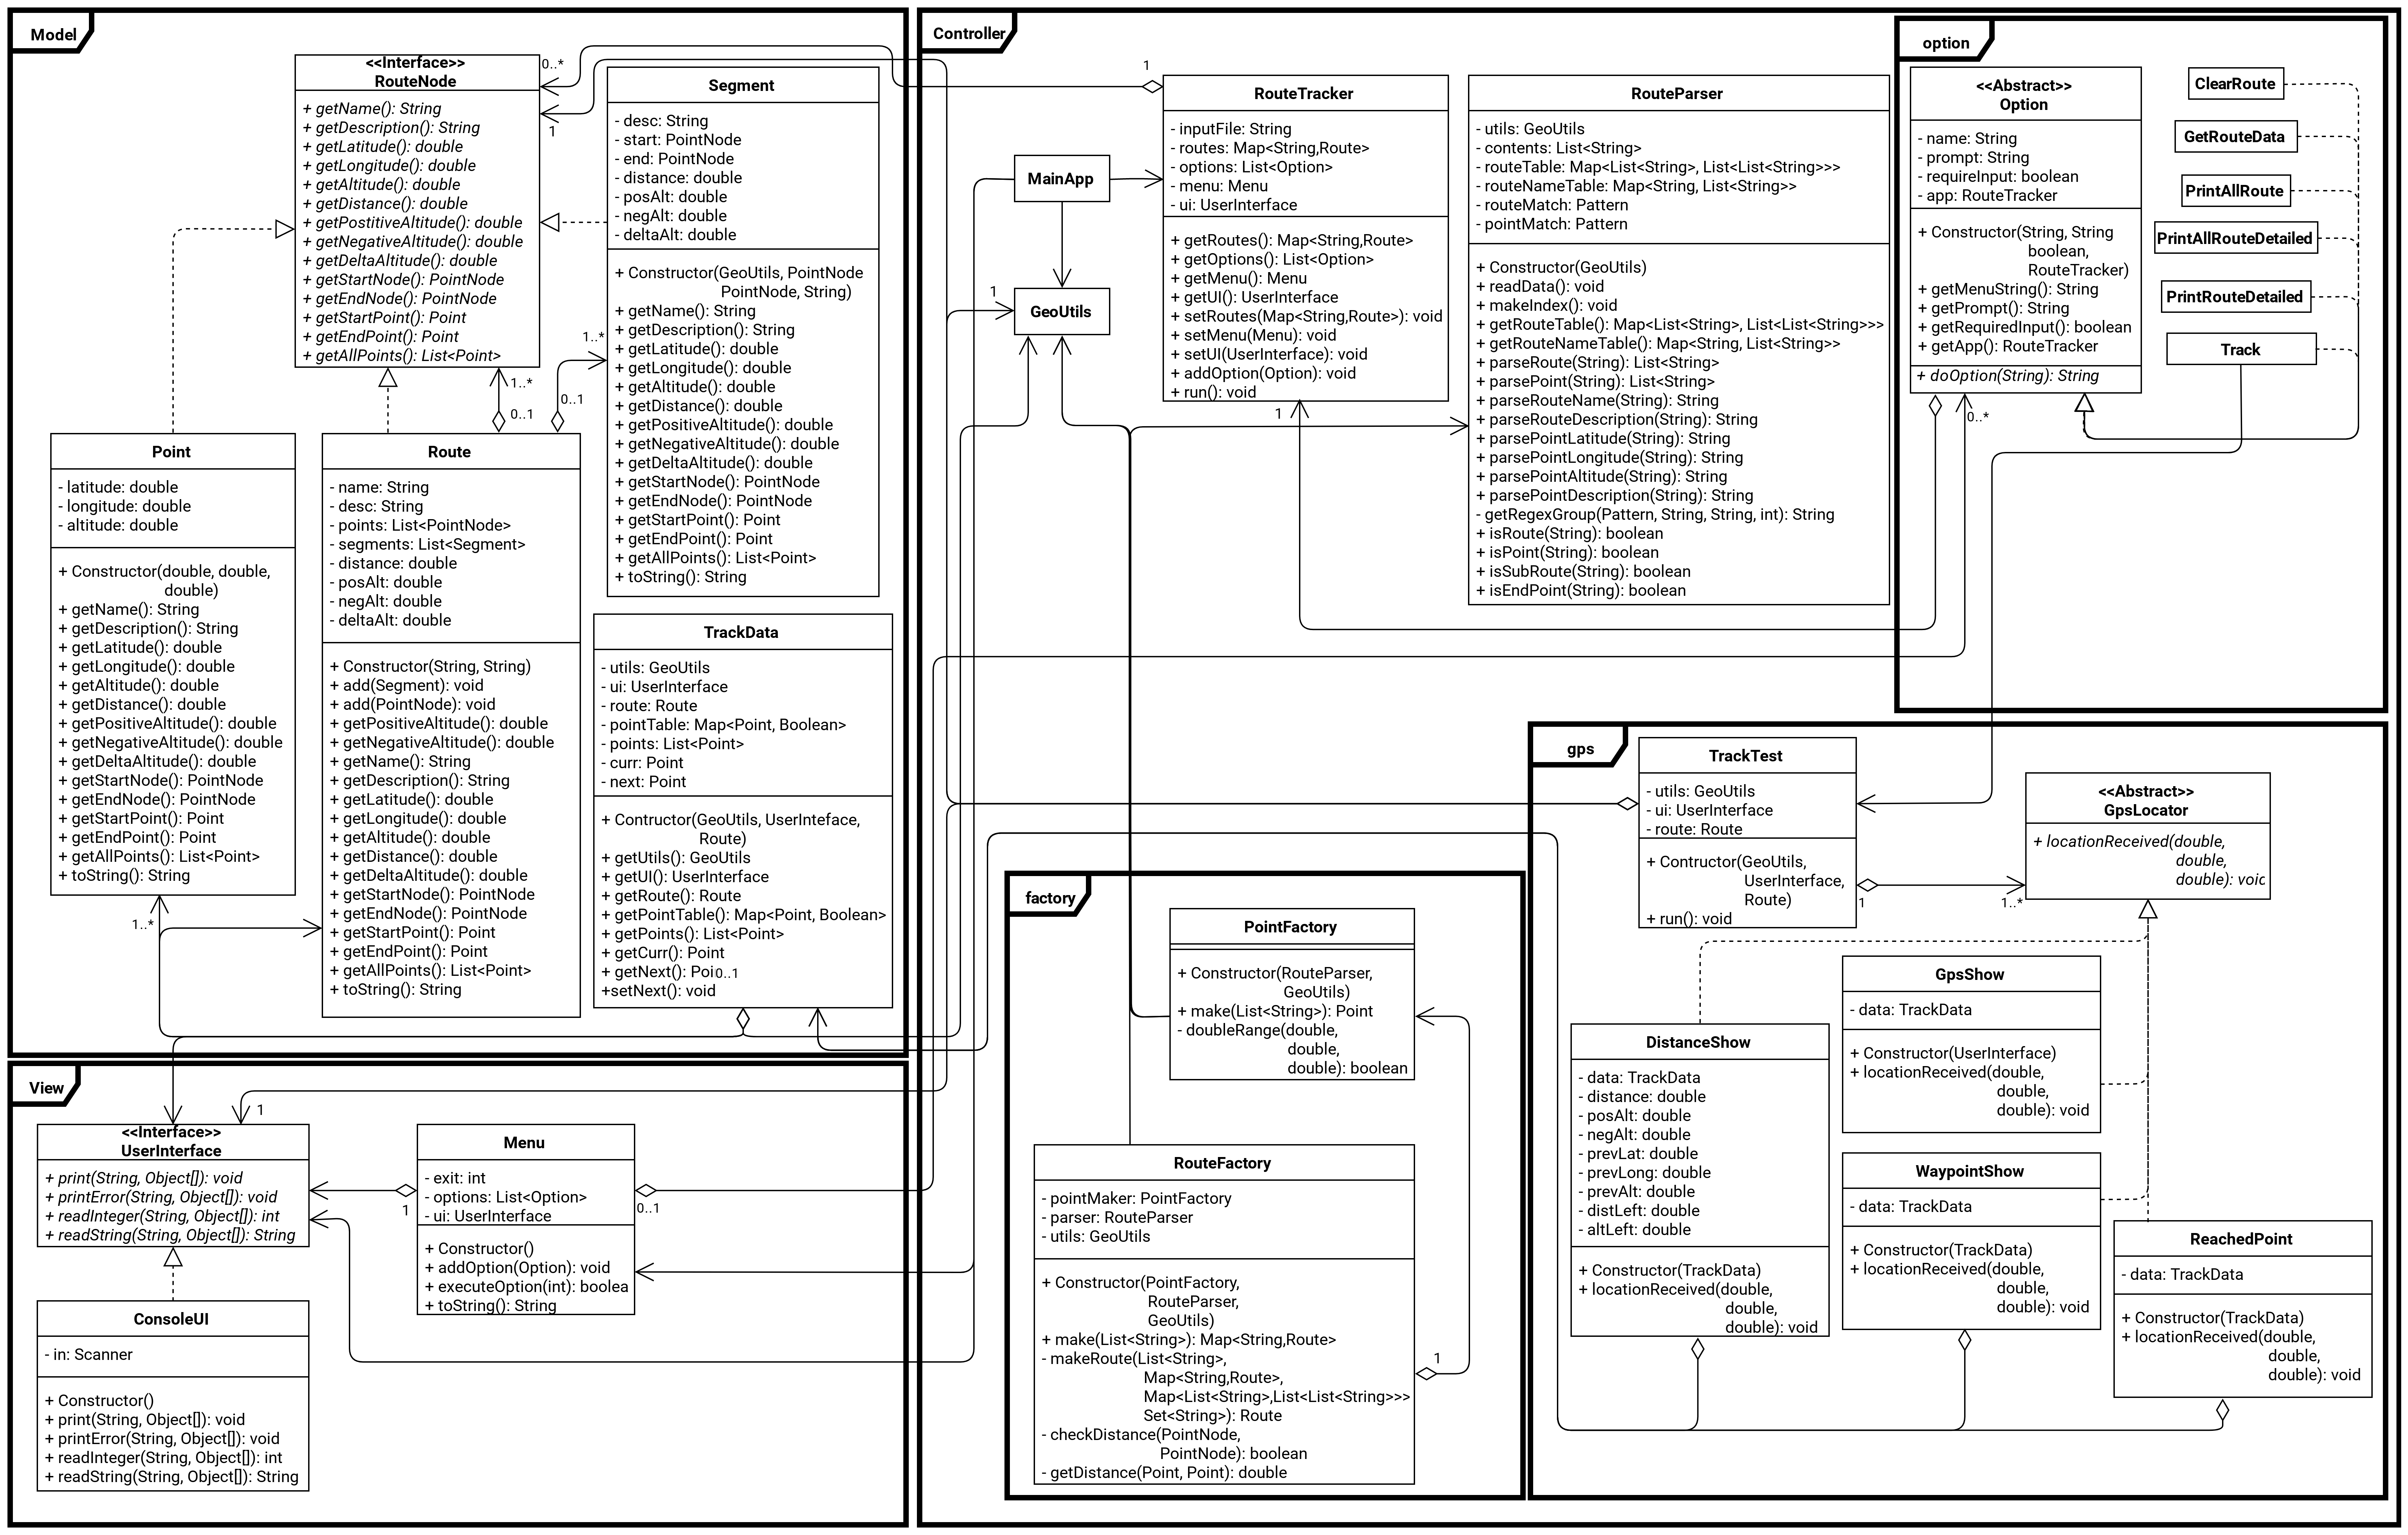
\includegraphics[
    angle=90,
    width=\textwidth,
    height=0.975\textheight,
    keepaspectratio
]{./docs/OOSE-Assignment-UML.png}

\newpage
\fancyhf[HL]{\footnotesize{Object Orientated Software Engineering - Discussion}}

\section{Discussion}
\subsection{Design Patterns}
\subsubsection{Route}

A route is defined as multiple points. A segment is within 2 points and routes
themselves can contain other routes, known as sub-routes. These sub-routes can
also contain sub-routes. Hence the sensible choice to represent routes is to
use a composite pattern. Composite pattern is useful for showing a hierachy of
objects, like a tree. In this case, we have an interface called
\code{PointNode}. \code{Point}, \code{Segment} and \code{Route} all implements
\code{PointNode} while \code{Route} can contain a collection of
\code{PointNode}. Hence, \code{Route} can store only \code{Point} objects or a
combination of \code{Point} and \code{Route}, thus allowing a \code{Route} to
contain a sub-route. It is important to point out that \code{Route} contains a
list of \code{Point} as well as a separate list of \code{Segment}. This is
needed because the description is tied to a segment. One solution would be to
have a map containing two points as a key and a string as a value. However,
this would require \code{Point} to have an implementation for \code{equals()}
and \code{hashCode()}. Additionally, more infomation such as distance between
the two points also needs to be stored. Thus, it would make more sense to have
a separate \code{Segment} class.

Another benefit of using a Composite pattern is that we can simply recursively
call methods in order to extract information from the route. For example, we
have a method that returns the distance of the route. Because all classes
implementing the \code{PointNode} interface, they would have to override the
\code{getDistance()} method. So when \code{getDistance()} is called within a
route, we would get the distance for every element in the collection of
\code{PointNode} objects, which can be either a \code{Point} or a \code{Route}.
Thus, we get the distance for the current route, including it's sub-routes.


\subsubsection{Options}

To be able to quickly add more functionality to the program, the Strategy
pattern is used. The \code{Menu} class holds a collection of \code{Option},
which is an abstract class that only has \code{doOption()} as the abstract
method. When the user selects an option, \code{Menu} fetches the option from a
list and calls the \code{doOption()} method. \code{Menu} does not know what
kind of \code{Option} it is, it just knows that it contains a \code{doOption()}
method which it calls. \code{doOption()} takes in a string and returns a
string. The imported string is the user's input, which could be an empty
string. The returned string is the output of the option, displayed by the
\code{Menu}.


\subsubsection{GpsLocator}

With the GpsLocator and tracking the user's location, some compromises are
made. The assignment specifications state that the actual implementation of the
\code{GpsLocator}'s template method is yet to be done. Thus it is not clear
whether GpsLocator contains the context of the program, such as the current
route selected, the user's last position, and which points on the route has
already been visited. Thus, in order to make this specific program to work,
each class that extends \code{GpsLocator} is given their own class fields
necessary for them to function. Classes like \code{GpsShow} does not need any
class fields since it's purpose is simple, but other classes like
\code{DistanceShow} or \code{ReachedPoint} is more complex, and needs to keep
track of the last position, or which point is marked visited. The downside to
this approach is that these classes would eventually need to be reworked so
that all the class fields are shared within each other. Another downside is
that there is no concrete way to test the \code{ReachedPoint} class as the user
would need to invoke that method manually, hence some assumptions are used
instead.


\subsection{Coupling, Cohesion, Reuse}

Coupling within this program is low because of the usage of polymorphism. The
program's user interface can easily be changed because there is an interface
called \code{UserInterface}. Currently, only \code{ConsoleUI} implements
\code{UserInterface}, but a GUI frontend can be written for this program as
long as it implements \code{UserInterface}. The most coupling this program has
is where a class uses another class's accessors or methods. Dependency
injection is heavily used as seen in the factory classes \code{PointFactory}
and \code{RouteFactory}. \code{RouteFactory} takes in a \code{PointFactory} in
order to create routes and \code{PointFactory} takes a \code{RouteParser} and
\code{GeoUtils}. No classes creates any new instance of another class in it's
constructor.

Cohesion within this program is high because each class has one defined
purpose. There is a total of 30 classes in this program. For example,
\code{PointFactory} and \code{RouteFactory} are separate classes, even though
the creation of routes relies heavily on points. \code{RouteTracker} class
contains the variables needed for the program. \code{RouteParser} only parses
the input file. Each source file contains a header that fully describes the
purpose of the source file.

Within the \code{RouteParser} class, there exists methods that extracts the
different information for a route or point string. In additional to this, there
also exist a method that gets all the route information and all the point
information. Originally, each method matches the line to the pattern, then
return the group index of the regex. The only line that is different to each is
the group index, thus to make use of code reuse, have a method called
\code{getRegexGroup()} which takes in an integer and returns the matched
string. Now the methods simply act as a wrapper of the \code{getRegexGroup()}
method, with the only difference being the group index.


\subsection{Alternative Designs}

In regards to the route structure, one could argue that a Decorator pattern can
be used to store routes. With a Decorator pattern, we could have \code{Route}
implementing a common interface. Then, have an abstract class \code{Point} that
implements same interface and have a sub class that extends the abstract class.
This allows a new \code{Point} to be added onto a \code{Route} class by
encapsulating it with the \code{Point}. One advantage with this approach is
that it would be easy to add new extendibility to \code{Route} by extending the
\code{Point} abstract class. However, this pattern is falls when adding
sub-routes to the \code{Route}. \code{Route} cannot extend \code{Point} because
then it would be too similar to the Composite pattern, thus more logic would be
needed to represent sub-routes.

In other parts of the program, implementing a State pattern to switch the
program's state from reading routes to tracking the user can be used instead of
having the tracking function within an option. By having a State pattern, it
will make it easy to implement various different state with a completely
different functionality using the same routes. The downside, at least for this
instance, would be that given the small scale of this program, a State pattern
would be unnecessary since there is only two states.


\end{document}
